%
% 2-tangentialvektoren.tex -- Tangentialvektoren
%
% (c) 2024 Prof Dr Andreas Müller
%
\section{Tangentialvektoren
\label{buch:koordinaten:section:tangentialvektoren}}
\kopfrechts{Tangentialvektoren}
Das elektrische Feld übt auf eine Testladung eine Kraft aus, die
proportional zur Ladung ist.
Diese Kräfte stellt man sich gerne als ein Vektorfeld vor, doch
in welchem Raum sind diese Vektoren zu finden?
Die Kraft verursacht eine Beschleunigung und verändert damit 
die Geschwindigkeit.
Als erstes muss daher der Geschwindigkeitsvektor konstruiert werden,
der tangential an die Bahnkurve der Testladung verläuft.
An dieser naheliegenden und üblichen Darstellung ist aber eigentlich
falsch, dass der Geschwindigkeitsvektor gar nicht im gleichen Raum
dargestellt werden kann.
Die Masseinheit der Komponenten des Geschwindigkeitsvektors ist
[Länge/Zeit], während die Koordinaten die Masseinheit [Länge] haben.
Solange man das Koordinatensystem und damit die Masseinheiten nicht
wechselt, mag die Konfusion in Grenzen bleiben.
Da aber alle Gesetzmässigkeiten auf eine koordinatensystemunabhängige
Art formuliert werden müssen, bedarf auch das Konzept des Tangentialvektors
einer Reevaluation.

%
% Kurven
%
\subsection{Kurven}
Für ein kartesisches Koordinatensystem in der Ebene ist klar, welche
Richtung man den Koordinatenachsen zuordnen kann.
Es ist üblich, die Koordinatenachsen als Vektoren in der Ebene
zu zeichnen.
Die Idee einer geraden Koordinatenachse ist nicht mehr anwendbar,
wenn beliebige Koordinatensystem verwendet werden sollen.
Bei der Umrechnung zwischen Koordinatensystemen entstehen unweigerlich
gekrümmte Koordinatenlinien.
Es braucht also etwas mehr Sorgfalt, die Idee der {\em Richtung}
Koordinatenunabhängig zu definieren.

\subsubsection{Differenzierbare Kurven}
Im Folgenden gehen wir on einer Menge $Y$ mit einer $n$-dimensionalen
differenzierbaren Struktur aus.
Statt uns auf die in der Einleitung angedeuteten gekrümmten
Koordinatenlinien zu beschränken, möchten wir beliebige Kurven
definieren.
Kurven sehen in der Umgebung eines Punktes wie die reelle Achse
$\mathbb{R}$ aus.
Tatsächlich können wir jedes Intervall $X=(a,b)\subset\mathbb{R}$ als
eine Menge mit einer differenzierbaren Struktur betrachten, indem
wir die Einbettung
\[
\varphi
\colon
X=(a,b) \hookrightarrow \mathbb{R}
:
x\mapsto x
\]
als Koordinatensystem verwenden.
Die Koordinatenwechselabbildung zu einem alternativen Koordinatensystem
auf dem Intervall ist eine streng monoton wachsende, differenzierbare
Funktion, deren Ableitung nirgends verschwindet.
In einem Punkt $x_0\in (a,b)$ sind Koordinatenwechsel daher sehr
einfach: Sie sind nur von 0 verschiedene Zahlen.
Diese Einfachheit erlaubt uns, zur Vereinfachung der Notation die Menge
$(a,b)$ mit den Koordinatenwerten zu identifizieren.

\begin{definition}[differenzierbare Kurve]
Eine {\em differenzierbare Kurve}
\index{differenzierbare Kurve}%
\index{Kurve, differenzierbar}%
ist eine differenzierbare Abbildung
\[
\gamma
\colon
X = (a,b) \to Y
:
t \mapsto \gamma(t).
\]
\end{definition}

Durch Zusammensetzen der Abbildung $\gamma$ mit einem Koordinatenssystem
$\varphi\colon X\to \mathbb{R}^n$ entsteht eine Abbildung 
\[
\varphi\circ\gamma
\colon
X=(a,b) \to \mathbb{R}^n
:
t \mapsto (\varphi^1\circ \gamma(t),\dots,\varphi^n\circ\gamma(t)),
\]
wobei jede Koordinate $\varphi^i\circ\gamma(t) = \varphi^i(\gamma(t))$
eine differenzierbare Funktion von $t$ ist.

\begin{beispiel}
Die Menge $Y=\mathbb{R}^2$ hat eine differenzierbare Struktur gegeben durch
das kartesische Koordinatensystem
\[
\varphi
\colon
Y\to\mathbb{R}^2
:
(x,y)\mapsto (x,y).
\]
Die Kurve 
\[
\gamma
\colon
\mathbb{R}\to Y
:
t\mapsto (\cos t, \sin t)
\]
ist der Einheitskreis in der Ebene.

Koordinatenwechsel auf dem Urbildbereich $(-\infty,\infty)$ sind durch
Funktionen $f\colon\mathbb{R}\to\mathbb{R}$ gegeben, deren Ableitung
nirgends verschwindet.
Nach dem Koordinatenwechsel ist die Kurven durch die Parametrisierung
\[
t \mapsto (\cos f(t),\sin f(t))
\]
gegeben.

Statt der kartesischen Koordinaten kann man mindestens auf der Teilmenge
$Y=X\setminus (0,0)$ Polarkoordinaten mit der Koordinatenabbildung $\psi$
verwenden.
Die Koordinatenumrechnung von Polarkoordinaten in kartesische Koordinaten
ist
\[
(\varphi, r) \mapsto (r\cos\varphi,r\sin\varphi)
\]
mit der Umkehrung
\[
(x,y) \mapsto \Bigl(\arctan\frac{y}{x},\sqrt{x^2+y^2}\Bigr),
\]
wobei die $\arctan$-Funktion etwas erweitert werden muss, wie es die
in den meisten Programmierbibliotheken durch die Funktion \texttt{atan2}
gemacht wird.

In Polarkoordinaten bekommt die Kurve $\gamma$ die Form
\[
t\mapsto \psi\circ\gamma(t)
=
(t, 1).
\]
Die zweite Koordinaten ist konstant und damit ganz offensichtlich 
differenzierbar.
Die erste Koordinate hat die Ableitung $1$.
\end{beispiel}

Eine Kurve in $Y$ ist also eine Abbildung $X\to Y$.
Sowohl in $X$ wie auch in $Y$ können beliebige Koordinatensysteme
gewählt werden.
Es ist nur sinnvoll über Objekte zu sprechen, welche in dem
Sinne unabhängig sind von der Wahl des Koordinatensystems, dass
auch Umrechnungsformeln zwischen den Koordinatensystemen bereitgestellt
sind.

% XXX Ableitung der Koordinaten

% XXX Koordinatenwechsel und Ableitung


\subsubsection{Tangentiale Kurven}
Das Beispiel illustriert, dass der Begriff der ``Richtung'' einer
Koordinatenachse nicht sinnvoll sein kann.
Im Wertebereich der Koordinatensysteme unterscheidet sich das Bild
der Kurve $\gamma$ grundsätzlich.
Im Koordinatensystem ist $\varphi\circ\gamma$ eine gekrümmte Kurve,
während sie im Polarkoordinatensystem in der Umgebung des Punktes
$(1,0)$ die Gerade $r=1$ ist.
Die Kurve durch einen Punkt von $Y$ kann also keine koordinatenunabhängig
Bedeutung haben, aber für die Richtung der Kurve in einem Punkt ist
dies möglich.
Es muss daher definiert werden, wann zwei Kurven die gleiche Richtung
in einem gemeinsamen Punkt haben.


%
% fig-kurve.tex
%
% (c) 2024 Prof Dr Andreas Müller
%
\begin{figure}
\centering
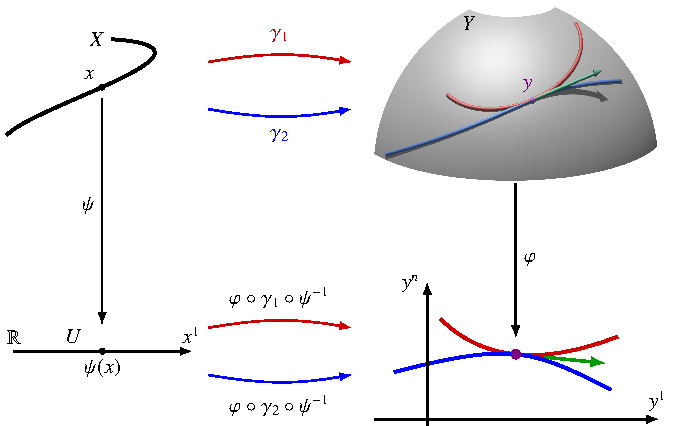
\includegraphics{chapters/020-koordinaten/images/kurve.pdf}
\caption{Die Kurven $\gamma_1$ und $\gamma_2$ sind tangential im
Punkt $y$, wenn $\gamma_1(x)=y=\gamma_2(x)$ und ausserdem die
Ableitungen der Zusammensetzungen $\varphi\circ\gamma_i\circ\psi^{-1}$
in $\psi(x)$ übereinstimmen.
Es ist nicht sinnvoll, von einem Tangentialvektor ``in $Y$'' (grün,
oben rechts) zu sprechen, erst durch das Koordinatensystem kann
das Konzept des Tangentialvektors konsistent definiert werden.
\label{buch:koordinaten:tangentialvektoren:fig:kurve}}
\end{figure}
%

\begin{definition}[tangentiale Kurven]
Zwei Kurven $\gamma_i\colon X\to Y$, $i=1,2$, sind
{\em tangential} im Punkt $y\in Y$, wenn
$\gamma_i(x) = y$, $i=1,2$, und
in jeder Karte
$\varphi\colon Y\to\mathbb{R}^n$ und für die Parametrisierung
$\psi\colon X\to \mathbb{R}$ mit Parameter $x^1\in\mathbb{R}$ 
im Punkt $\psi(x)$ die Ableitungen der Abbildungen
\[
\varphi
\circ
\gamma_i
\circ
\psi^{-1}
\colon
U\to\mathbb{R}^n
\]
übereinstimmen, d.~h.
\begin{equation}
\frac{d}{dx^1}
\bigl(\varphi\circ\gamma_1\circ\psi^{-1}\bigr)(\psi(x))
=
\frac{d}{dx^1}
\bigl(\varphi\circ\gamma_2\circ\psi^{-1}\bigr)(\psi(x))
\label{buch:koordinaten:tangentialvektoren:eqn:tangential}
\end{equation}
für $x^1=\psi(x)$.
\end{definition}

%
% Tangentialvektoren
%
\subsection{Tangentialvektoren}

%
% Koordinatenlinien
%
\subsection{Koordinatenlinien}



